\documentclass[10pt, a4paper, english]{article}

%% packages
\usepackage[T1]{fontenc}
\usepackage{pgfplotstable} % include graphics
\usepackage{tikz}
\usetikzlibrary{trees, arrows, shapes.geometric, positioning}
\usepackage{tikzpeople}
\usepackage{forest}
\usepackage{standalone}
\usepackage{natbib}
\usepackage{geometry}
\usepackage{helvet} % Helvetica aka Arial
\usepackage[normalem]{ulem} % underline
\usepackage[affil-it]{authblk} 
\usepackage{mwe}

%% set geometry
\geometry{
 a4paper,
% total={170mm,257mm},
 top = 20mm,
 left = 20mm,
 right = 20mm,
 bottom = 20mm,
 bindingoffset = 0cm % gutter
}

%% renew commands
\renewcommand{\familydefault}{\sfdefault}
\renewcommand\Authfont{\fontsize{12}{14.4}\selectfont}
\renewcommand\Affilfont{\fontsize{10}{10.8}\selectfont}

%\renewcommand\email{\fontsize{10}{10}\selectfont}

\begin{document}

\title{\textbf{Standartox – a tool for assessing the risk of chemicals}}

\author{\uline{Scharmüller, Andreas}\textsuperscript{1}}
\author{Schreiner, Verena C.\textsuperscript{1}}
\author{Schäfer, Ralf B. \textsuperscript{1}}
\date{\vspace{-5ex}}

\affil{Institute for Environmental Sciences, University Koblenz-Landau, 76829 Landau in der Pfalz, Germany}

%\href{mailto:scharmueller@uni-landau.de}{scharmueller@uni-landau.de}
\maketitle

\section{Introduction}
An increasing number of chemicals such as pharmaceuticals, pesticides and synthetic hormones are in daily use all over the world. In Europe alone, some 100,000 chemicals are estimated to be in current use, whereof 30,000 are produced in quantities larger than one ton per year \citep{breithaupt_costs_2006}. Except for pesticides that are released into the environment deliberately, most chemicals enter the environment as a result of their use through different paths (e.g. atmospheric emission and deposition or discharge through wastewater) \citep{schwarzenbach_challenge_2006}. In the environment, chemicals can adversely affect populations and communities and in turn related ecosystem functions. Pollution with man-made chemicals has been identified as one of three major environmental problems for which research gaps hamper the derivation of planetary boundaries, i.e. thresholds beyond which irreversible state shifts may occur \citep{steffen_planetary_2015}. Even highly regulated chemical compounds such as pesticides have been shown to cause strong adverse effects on organisms, such as birds \citep{hallmann_declines_2014} or fish \citep{yamamuro_neonicotinoids_2019}, questioning the current regulation efforts \citep{schafer_future_2019}. To evaluate the risks from chemicals for ecosystems data on their toxicity, which is typically produced in standardised ecotoxicological laboratory tests is required \citep{malaj_organic_2014, morrissey_neonicotinoid_2015}. Similarly, permissible environmental concentrations are often derived from these test data, typically by a combination with safety factors to account for uncertainties. Given that data sets with large numbers of analysed chemicals are becoming increasingly available, ecotoxicity data are pivotal for regulatory risk assessment and science. To date, only few initiatives exist that aim to create a public resource of harmonized and quality controlled ecotoxicological data, such as the United States Environmental Protection Agency ECOTOXicology knowledgebase (EPA ECOTOX) \citep{elonen_ecotoxicology_2018}, the German Environmental Agency's Information System Ecotoxicology and Environmental Quality Targets (ETOX) \citep{umweltbundesamt_etox_2019} or the Pesticide Property Data Base (PPDB) \citep{lewis_international_2016}. The former two compile all available test results into a database. However, for many chemicals, multiple ecotoxicity values are available for the same test organism, which can vary strongly. Hence, these databases can contain multiple entries for the same test without quality information and with different units, hampering reproducible science if different values are selected for studies. The PPDB database is confined to pesticides and provides harmonised and quality controlled data for a few selected test organisms, thereby ignoring vast amounts of data for other species and chemicals. Moreover, data analyses often require links to additional data resources, for example to append additional chemical and species information (e.g. chemical properties, habitat of species), which calls for more automated procedures. We developed Standartox, a tool and database that aims to overcome the limitations of other databases by continuously incorporating the ever-growing number of test results in an automated process workflow that ultimately leads to single aggregated data point for a specific chemical-organism test combination, representing the toxicity of a chemical. Hence, Standartox provides the basis for reproducible science and combines information from different sources to simplify the derivation of more advanced risk indicators such as Species Sensitivity Distributions (SSD) and Toxic Units (TU), which represent two prominent concepts to assess effects on organisms in ecotoxicology \citep{posthuma_species_2002, kefford_definition_2011}. Besides aggregating ecotoxicological test results, Standartox provides a concise overview of the status of tested chemicals, allowing the identification of potential research gaps. Standartox comes with two front-ends, a web application (APP) (www.standartox.uni-landau.de) and a R package, which accesses a application programming interface (API) providing convenience structures and thereby largely reducing processing time for users.

\section{Methods}
Standartox downloads the EPA ECOTOX data base and builds it locally. It then extracts CAS numbers and taxonomic nomenclatures to query additional information from chemical and taxonomic specific data bases, respectively. Subsequently, measurement units are harmonized, filter parameters are created and a final data set is created and exported.

\section{Results and Discussion}
The exported object can then be accessed by a web application or an R-package to retrieve filtered and aggregated test results, as a comma-separated values (csv) file or directly within R. Users can filter the test data by CAS numbers, chemical classes (e.g. herbicides, metals), taxa, habitat-specific parameters (e.g. freshwater), test duration as well as effect (e.g. mortality, growth) and endpoint (e.g. EC\textsubscript{50}, NOEC, LOEC) groups. Furthermore test results can be aggregated by the geometric mean. On top of filtering the data, Standartox provides means to aggregate results from multiple ecotoxicological tests to retrieve single exposure endpoints for specific chemical, taxon and test parameter combinations. Test results for each chemical in the filtered data set are thereby aggregated by calculating the minimum, the geometric mean or the maximum. Standartox returns then a filtered and an aggregated data set (Figure \ref{fig:stx-organigram}). Besides, Standartox allows users to access older versions of the data base as well and is created as open source software and therefore a fully reproducible method. Standartox constitutes not only a one-time compiled data set but rather a scalable method that can steadily incorporate new ecotoxicological test data in an automated manner, allowing for constant improvement of toxicity estimations over time. To, date Standartox provides access to more than 605,000 test results and its aggregates. In order to asses the validity of the Standartox aggregation approach, we compared Standartox results with effect values from the PPDB (n=3601) for the same chemicals (Figure \ref{fig:standartox_ppdb_diff}). This showed that 91.3\% of the Standartox values diverge by less than a factor of ten from the PPDB values. Considering only Standartox values for which at least five or ten tests were aggregated the value increases to 91.7\% and 93.4\%, respectively.



\begin{figure}
    \centering
    \begin{minipage}{0.45\textwidth}
        \centering
        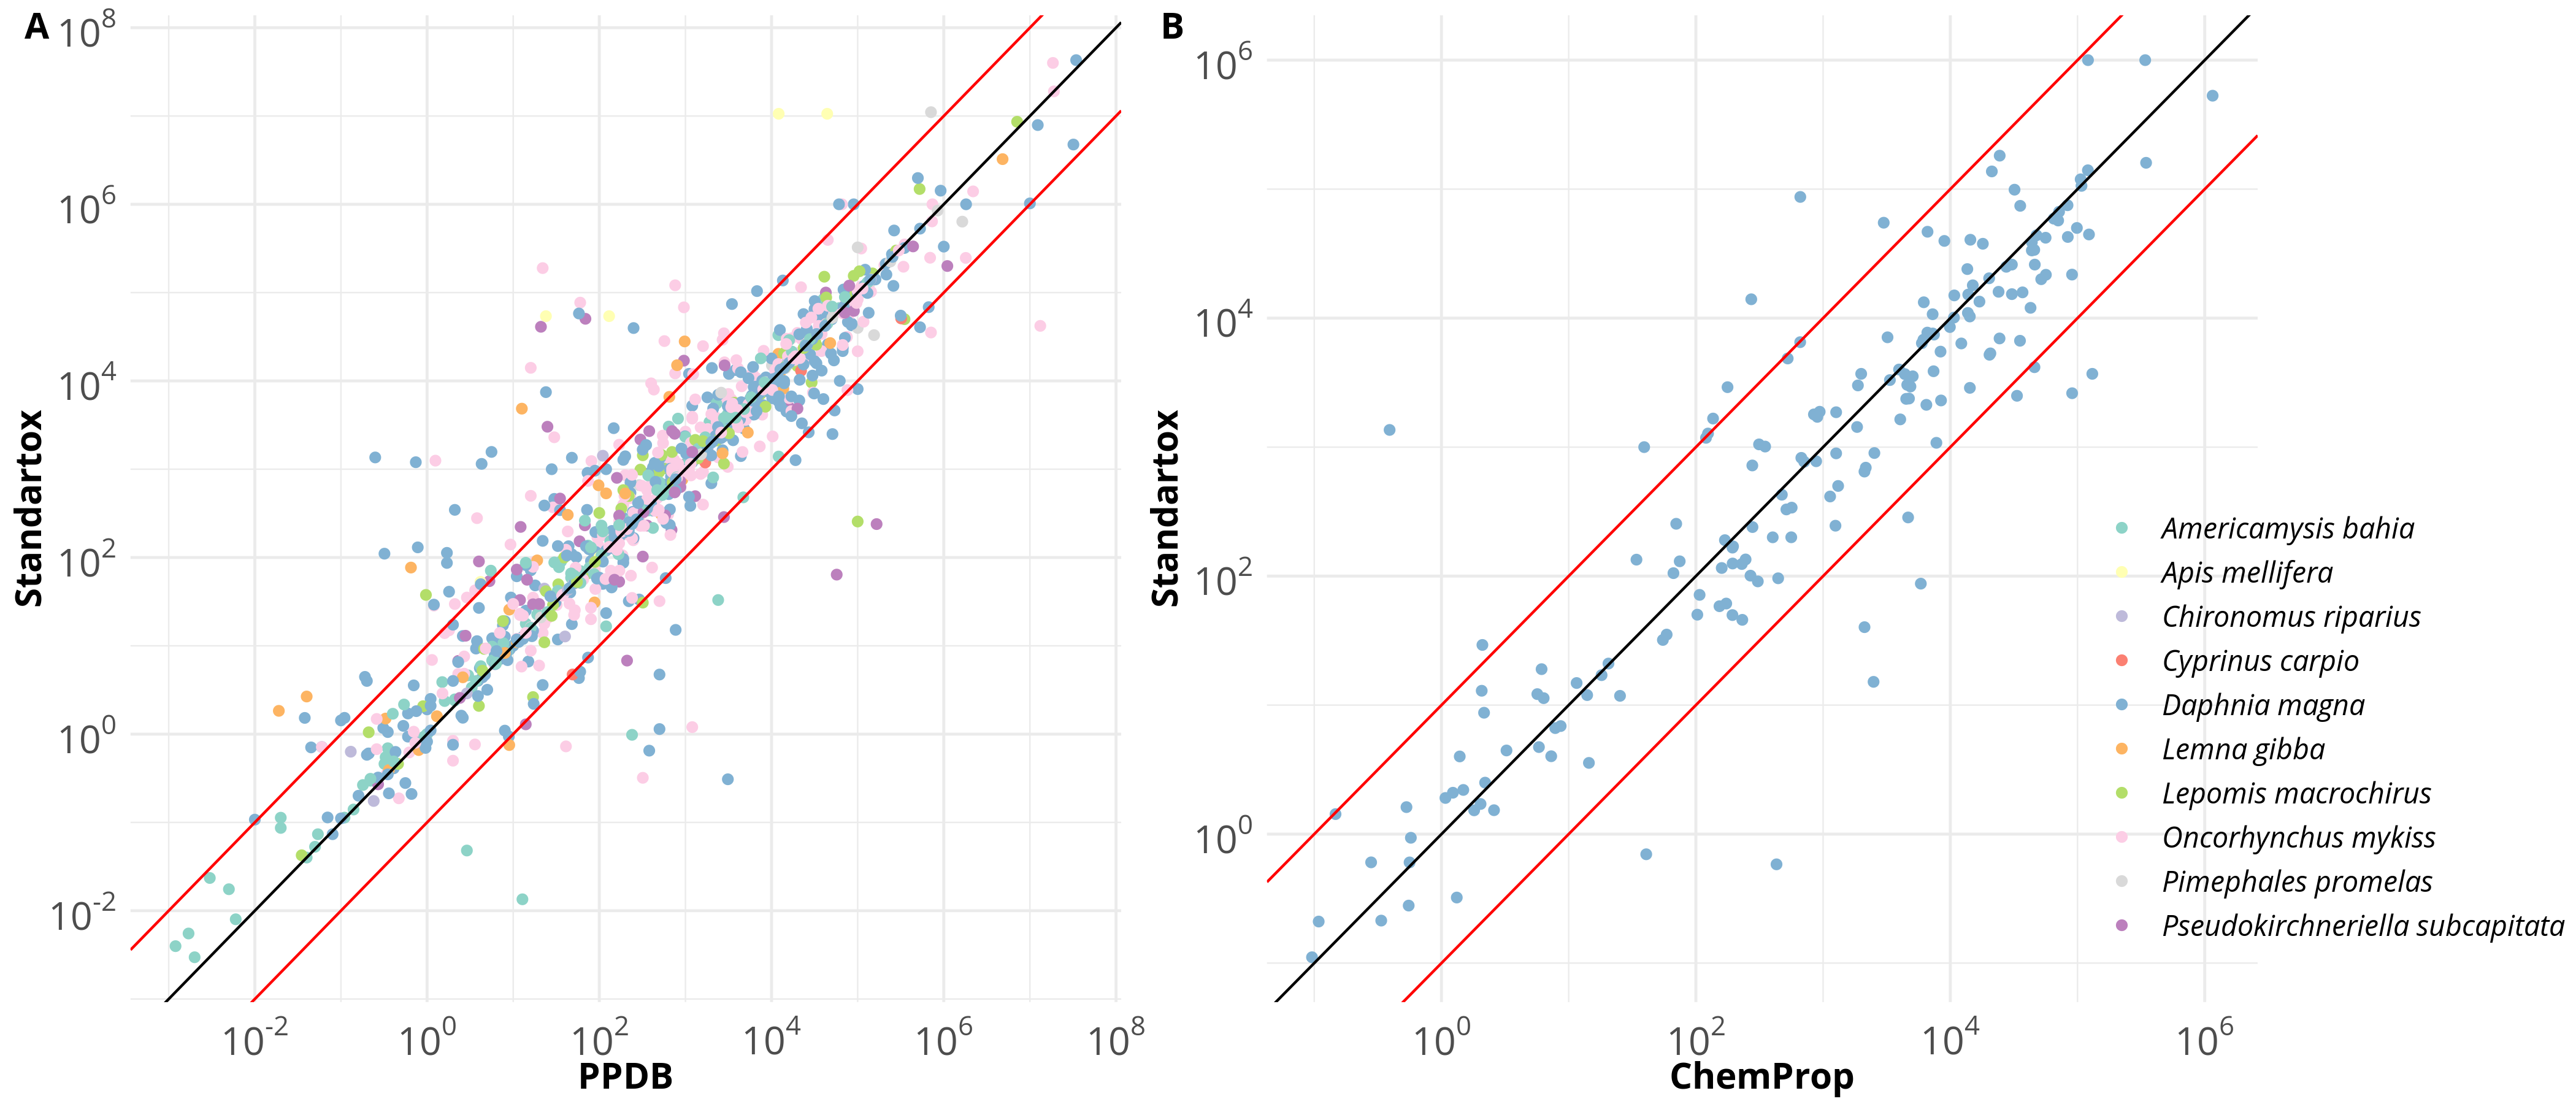
\includegraphics[width=0.9\textwidth]{article/figures/gg_ppdb_stan_compare_continous.png}
        \caption{Comparison between Standartox and PPDB values. The black line marks exact coherence and red lines mark a divergence of a factor of 10. Compared organism groups are color coded.}
    \end{minipage}\hfill
    \begin{minipage}{0.45\textwidth}
        \centering
        \includestandalone[width=0.9\textwidth]{article/tikz/standartox_organigram} % second figure itself
        \caption{Organigram of Standartox. Users can access Standartox via a web application or an R-package.}
    \end{minipage}
\end{figure}

\bibliographystyle{apalike}
\bibliography{refs/references-standartox.bib}

\end{document}